\documentclass[11pt]{article}

%%%%%%%%%%%%%%Include Packages%%%%%%%%%%%%%%%%%%%%%%%%%%
\usepackage{xcolor}
\usepackage{mathtools}
\usepackage[a4paper, total={6in, 8in}, margin=1.25in]{geometry}
\usepackage{amsmath}
\usepackage{amssymb}
\usepackage{paralist}
\usepackage{rsfso}
\usepackage{amsthm}
\usepackage{wasysym}
\usepackage[inline]{enumitem}
\usepackage{hyperref}
\usepackage{tocloft}
\usepackage{titlesec}
\usepackage{colortbl}
\usepackage[american]{circuitikz}
%%%%%%%%%%%%%%%%%%%%%%%%%%%%%%%%%%%%%%%%%%%%%%%%%%%%%%%%



\begin{document}
\Large \noindent \textbf{Physics 5C Midterm 2 Review Session}\\
\normalsize
Department of Physics and Astronomy, UCLA\\
%\noindent TA: Jinyan Miao (jnmiu@ucla.edu)\\
%Office hours: Thursday 10-11 AM $\&$ 1-2 PM at PAB 2-429\\
%Tutoring center hours: Friday 2-3 PM at PAB 2-429 (Zoom room also available)\\
\noindent\rule{8cm}{0.4pt}\\

\noindent\textbf{Problem 1}: There is a circuit on the lab table.\\

A battery of emf $\varepsilon$ is connected in series with a resistor $R_1=R$. After that resistor, the circuit splits into two parallel branches. One branch contains a resistor of resistance $R_2 = 2R$. The other branch contains another resistor $R_3 = 3R$. The two branches then rejoin and return to the battery. In this problem, assume that the wires are ideal and have no resistance, and solve the problem symbolically.\\

\noindent\textbf{Part (a)} Draw an equivalent circuit diagram. \\

\noindent\textbf{Part (b)} Find the equivalent resistance in this circuit.\\

\noindent\textbf{Part (c)} Find the current going through the battery, and the current going through $R_1$.\\ 

\noindent\textbf{Part (d)} Find the voltage drop across $R_1$, and the voltage drops across $R_2$ and $R_3$.\\

\noindent\textbf{Part (e)} Find the current $I_2$ going through $R_2$, and $I_3$ going through $R_3$.\\

\noindent\textbf{Part (f)} Find the energy dissipated by each of the resistors in $10$ seconds.\\

\noindent\textbf{Part (g)} Now if we replace $R_3$ with another resistor $R_4$ that has the same resistance, is made out of the same material (and thus has the same resistivity), but is twice as long as $R_3$, find the cross-sectional area of $R_4$ compared to that of $R_3$. Label the cross-sectional area of $R_3$ as $A_3$.\\

\newpage
\noindent\textbf{Problem 2} Evil Jinyan sneaked into the lab and replaced $R_1$ in the circuit with a capacitor $C_1$ that has a capacitance $C$. The capacitor is initially uncharged.\\

\noindent\textbf{Part (a)} Draw an equivalent circuit diagram immediately after the circuit is completed. \\

\noindent\textbf{Part (b)} Find the current going through $R_2$ and $R_3$ right after the circuit is completed.\\

\noindent\textbf{Part (c)} Find the current going through $R_2$ and $R_3$ a decade after the circuit is completed. By that time, the capacitor $C_1$ should have been fully charged. \\

\noindent\textbf{Part (d)} Find the voltage across the capacitor a decade after the circuit is completed.\\

\noindent\textbf{Part (e)} Find the total energy stored in $C_1$ when the capacitor is uncharged.\\

\noindent\textbf{Part (f)} Find the total energy stored in $C_1$ when the capacitor is fully charged.\\

\noindent\textbf{Part (g)} Jinyan finds that $C_1$ is actually a parallel-plate capacitor. Help him compute the amount of charge stored on one of the plates of $C_1$ when $C_1$ is fully charged. \\

\noindent\textbf{Part (h)} If Jinyan inserts some mysterious material (with $\kappa > 1$) in between the two plates of $C_1$, what will happen to the amount of charge stored on the plates and the amount of energy stored in the capacitor when it is fully charged?\\

\noindent\textbf{Part (i)} So far we have assumed that the battery has zero \textit{internal} resistance. Now assume the same setup, but the battery has internal resistance $r$. Find the current going through the battery right after the circuit is completed.\\

\noindent\textbf{Part (j)} Assume the battery has internal resistance $r$. Find the voltage across the battery terminals right after the circuit is completed.\\

\noindent\textbf{Part (k)} Jinyan replaces all resistors in the circuit with capacitors: $R_1$ is replaced by $C_1 = C$, $R_2$ is replaced by $C_2 = 2C$, and $R_3$ is replaced by $C_3 = 3C$. Find the equivalent capacitance of all the capacitors combined. 

\vfill
\hfill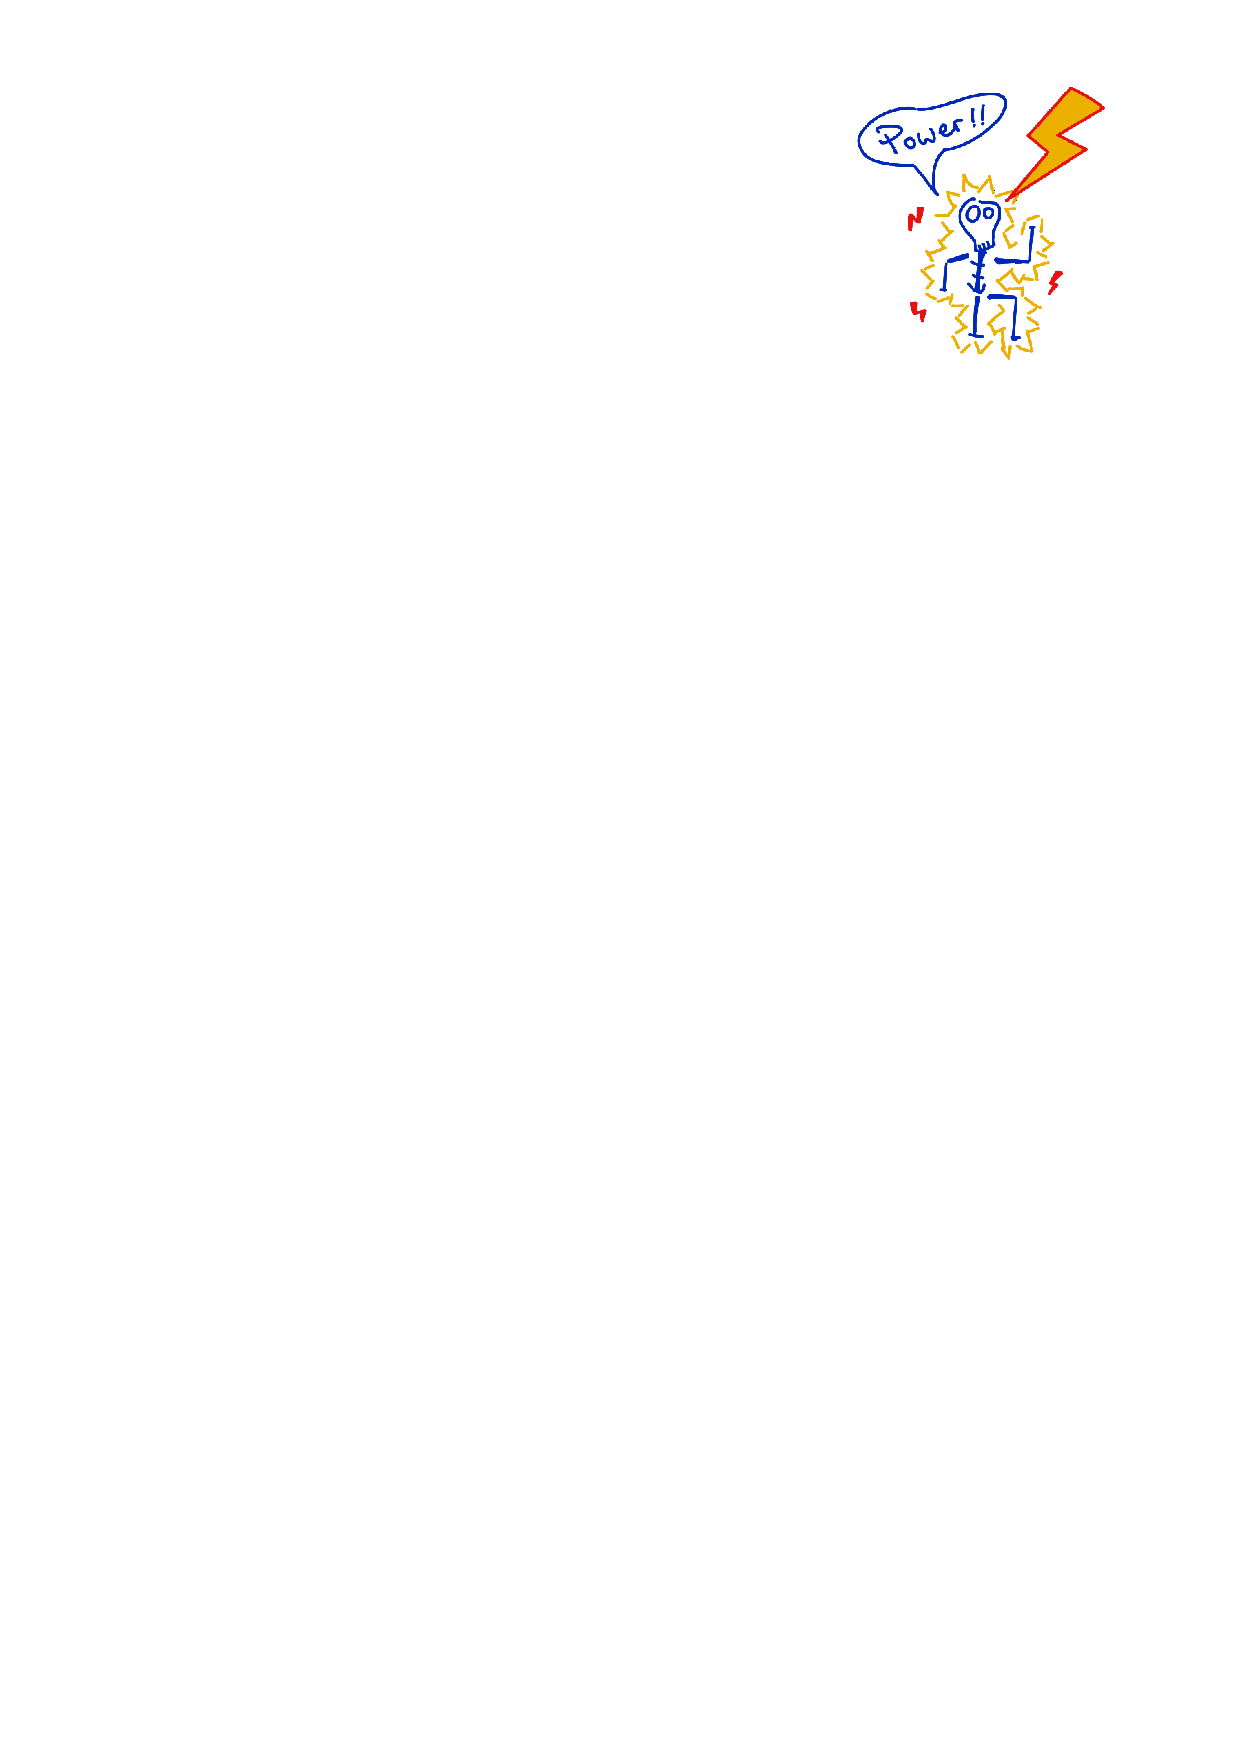
\includegraphics[scale=0.8]{shock}

\newpage
\section*{Problem 1}

The first thing we should do in this problem is to identify the structure of the circuit. Current from the battery must first pass through $R_1$, then it reaches a junction and splits into two branches, one through $R_2$ and the other through $R_3$, and finally the two branches recombine and go back to the battery. Therefore the circuit is $R_1 \text{ in series with } (R_2 \parallel R_3)\,.$\\

\noindent\textbf{Part (a)} Based on the argument above, the equivalent circuit diagram is
\begin{center}
\begin{circuitikz}[scale=0.95, transform shape]
\draw
(0,0) to[battery1,invert,l=$\varepsilon$] (0,6)
(0,6) -- (5,6) -- (5,5.5) to[R,l=$R$] (5,3.5)
(5,3.5) -- (4,3.5) to[R,l=$2R$] (4,0.5) -- (5,0.5)
(5,3.5) -- (6,3.5) to[R,l=$3R$] (6,0.5) -- (5,0.5)
(5,0.5) -- (5,0) -- (0,0);
\end{circuitikz}
\end{center}
That is, $R_1$ is in series with the parallel combination of $R_2$ and $R_3$.\\

\noindent\textbf{Part (b)} Since $R_2$ and $R_3$ are in parallel, we first combine them,
\begin{align*}
\frac{1}{R_{23}} = \frac{1}{R_2}+\frac{1}{R_3}
= \frac{1}{2R}+\frac{1}{3R}
= \frac{5}{6R}\,.
\end{align*}
Therefore,
\begin{align*}
R_{23} = \frac{6R}{5}\,.
\end{align*}
Now this parallel combination $R_{23}$ is in series with $R_1=R$, so the total equivalent resistance of the circuit is
\begin{align*}
R_{\text{eq}} = R_1 + R_{23}
= R+\frac{6R}{5}
= \frac{11R}{5}\,.
\end{align*}

\noindent\textbf{Part (c)} The current going through the battery is found from Ohm's law using the equivalent resistance,
\begin{align*}
I_{\text{battery}} = \frac{\varepsilon}{R_{\text{eq}}}
= \frac{\varepsilon}{11R/5}
= \frac{5\varepsilon}{11R}\,.
\end{align*}
Since the resistor $R_1$ is in series with the battery before the junction, it carries the same current as the battery. Thus
\begin{align*}
I_1 = I_{\text{battery}} = \frac{5\varepsilon}{11R}\,.
\end{align*}

\noindent\textbf{Part (d)} The voltage drop across $R_1$ is found, using Ohm's law again,
\begin{align*}
V_1 = I_1R_1
= \left(\frac{5\varepsilon}{11R}\right)R
= \frac{5\varepsilon}{11}\,.
\end{align*}
Since the battery provides total voltage $\varepsilon$, and $R_1$ is in series with the parallel part, the remaining voltage must be across the parallel part,
\begin{align*}
V_{23} = \varepsilon - V_1
= \varepsilon - \frac{5\varepsilon}{11}
= \frac{6\varepsilon}{11}\,.
\end{align*}
Because $R_2$ and $R_3$ are in parallel, they have the same voltage drop. Therefore,
\begin{align*}
V_2 = V_3 = \frac{6\varepsilon}{11}\,.
\end{align*}

\noindent\textbf{Part (e)} Now use Ohm's law on each branch. For resistor $R_2 = 2R$,
\begin{align*}
I_2 = \frac{V_2}{R_2}
= \frac{(6\varepsilon/11)}{2R}
= \frac{3\varepsilon}{11R}\,.
\end{align*}
For resistor $R_3 = 3R$,
\begin{align*}
I_3 = \frac{V_3}{R_3}
= \frac{(6\varepsilon/11)}{3R}
= \frac{2\varepsilon}{11R}\,.
\end{align*}
As a quick check,
\begin{align*}
I_2 + I_3 = \frac{3\varepsilon}{11R}+\frac{2\varepsilon}{11R}
= \frac{5\varepsilon}{11R}
= I_{\text{battery}}\,,
\end{align*}
which agrees with what we found in part (d).\\

\noindent\textbf{Part (f)} The energy dissipated by a resistor in time $\Delta t$ is
\begin{align*}
E = P\Delta t\,.
\end{align*}
Here $\Delta t = 10$ seconds. There are many ways to compute the power, for example $P=IV$, $P=I^2R$, or $P=V^2/R$. They are all related by Ohm's law: If you apply Ohm's law to one of them, you can get one of the other ones. Let us use $P=IV$ in this part.\\

For resistor $R_1$,
\begin{align*}
E_1 = I_1V_1(10\,\text{s})
= \left(\frac{5\varepsilon}{11R}\right)\left(\frac{5\varepsilon}{11}\right)(10)
= \frac{250\varepsilon^2}{121R}\,\text{J}\,.
\end{align*}

For resistor $R_2$,
\begin{align*}
E_2 = I_2V_2(10\,\text{s})
= \left(\frac{3\varepsilon}{11R}\right)\left(\frac{6\varepsilon}{11}\right)(10)
= \frac{180\varepsilon^2}{121R}\,\text{J}\,.
\end{align*}

For resistor $R_3$,
\begin{align*}
E_3 = I_3V_3(10\,\text{s})
= \left(\frac{2\varepsilon}{11R}\right)\left(\frac{6\varepsilon}{11}\right)(10)
= \frac{120\varepsilon^2}{121R}\,\text{J}\,.
\end{align*}

\noindent\textbf{Part (g)} The resistance of a conductor is
\begin{align*}
R = \frac{\rho L}{A}\,,
\end{align*}
where $\rho$ is the resistivity, $L$ is the length, and $A$ is the cross-sectional area of the conductor. The new resistor $R_4$ is made of the same material as $R_3$, so the resistivity stays the same. We are also told that $R_4$ has the same resistance as $R_3$, but twice the length. Thus
\begin{align*}
R_3 = \frac{\rho L_3}{A_3}\,,\qquad
R_4 = \frac{\rho (2L_3)}{A_4}\,.
\end{align*}
Since $R_4=R_3$,
\begin{align*}
\frac{\rho (2L_3)}{A_4} = \frac{\rho L_3}{A_3}\,.
\end{align*}
Canceling the common factors $\rho$ and $L_3$, we get
\begin{align*}
\frac{2}{A_4} = \frac{1}{A_3}\,,
\end{align*}
so
\begin{align*}
A_4 = 2A_3\,.
\end{align*}
Therefore the new resistor must have twice the cross-sectional area of $R_3$ in order to keep the same resistance while being twice as long.\\

\newpage
\section*{Problem 2}

Now resistor $R_1$ is replaced by a capacitor $C_1$ that is initially uncharged. The key fact for this entire problem is the following: An uncharged capacitor behaves like a wire immediately after the circuit is completed, but after a very long time it behaves like an open circuit (a break in the wire). Once you keep this picture in mind, the whole problem becomes very manageable, and we just need to consider two limits separately.\\

\noindent\textbf{Part (a)} Right after the circuit is completed, $C_1$ is uncharged, so it behaves like a wire. Therefore the equivalent circuit at $t=0$ is just a battery directly connected across the parallel combination of $R_2$ and $R_3$. Here we can draw the equivalent circuit by simply replacing the capacitor with a wire.
\begin{center}
\begin{circuitikz}[scale=0.95, transform shape]
\draw
(0,0) to[battery1,invert,l=$\varepsilon$] (0,4)
(0,4) -- (3,4) -- (3,3.5) -- (2,3.5) to[R,l=$2R$] (2,0.5) -- (3,0.5) -- (3,0) -- (0,0)
(3,3.5) -- (4,3.5) to[R,l=$3R$] (4,0.5) -- (3,0.5);
\end{circuitikz}
\end{center}
So at $t=0$, the capacitor can be ignored and the circuit is simply $R_2$ in parallel with $R_3$.\\

\noindent\textbf{Part (b)} Since $R_2$ and $R_3$ are directly across the battery right after the circuit is completed, each branch has voltage $\varepsilon$ across it. Therefore,
\begin{align*}
I_2(t=0) = \frac{\varepsilon}{R_2}
= \frac{\varepsilon}{2R}\,,
\end{align*}
and
\begin{align*}
I_3(t=0) = \frac{\varepsilon}{R_3}
= \frac{\varepsilon}{3R}\,.
\end{align*}

\noindent\textbf{Part (c)} A decade later, the capacitor is fully charged. A fully charged capacitor behaves like an open circuit, and here the capacitor sits in series before the two resistor branches. Therefore the circuit is broken and no current can flow anywhere in the loop. Hence
\begin{align*}
I_2(t\to \infty)=0\,\text{A}\,,\qquad
I_3(t\to \infty)=0\,\text{A}\,.
\end{align*}

\noindent\textbf{Part (d)} At long time, since the current through $R_2$ and $R_3$ is zero, the voltage drop across each resistor is also zero. Therefore the entire battery emf must appear across the capacitor,
\begin{align*}
V_C(t\to \infty)=\varepsilon\,.
\end{align*}

\noindent\textbf{Part (e)} When the capacitor is uncharged, the voltage across it is zero. The stored energy in a capacitor is
\begin{align*}
U_c = \frac{1}{2}CV^2\,.
\end{align*}
It is written in this form (instead of other forms that could be used to calculate the capacitor energy) because $C$ is given in the problem and we can find the voltage $V$ across the capacitor easily. At the initial time, the capacitor is uncharged, thus the voltage across it must be zero (since $C=Q/V$ for capacitance, then $V=Q/C$, so for an uncharged capacitor $Q=0$, we have $V = 0$),
\begin{align*}
U_{c,\text{uncharged}} = \frac{1}{2}C(0)^2 = 0\,\text{J}\,.
\end{align*}



\noindent\textbf{Part (f)} When the capacitor is fully charged, we just found from part (d) that the voltage across it is $\varepsilon$. Therefore,
\begin{align*}
U_{c,\text{charged}} = \frac{1}{2}C\varepsilon^2\,.
\end{align*}

\noindent\textbf{Part (g)} The amount of charge stored on one of the plates is related to capacitance and voltage by
\begin{align*}
Q=CV\,.
\end{align*}
Since the capacitor is fully charged and has voltage $\varepsilon$ across it,
\begin{align*}
Q = C\varepsilon\,.
\end{align*}


\noindent\textbf{Part (h)} Now a dielectric with $\kappa >1$ is inserted between the plates. The dielectric material changes the capacitance of the capacitor, and it does not affect the voltage across the capacitor. This is because the battery is the source of voltage in the circuit. If the battery and other resistive components in the circuit do not change, the voltage across the capacitor should not change. As you can verify, in our calculation of the voltage drop across the capacitor in part (d), it does not depend on the capacitance of the capacitor. Thus $V_C(t\to \infty)=\varepsilon$ is unchanged.
However, due to the dielectric, the capacitance becomes
\begin{align*}
C'=\kappa C\,.
\end{align*}
Therefore the stored charge becomes
\begin{align*}
Q'  =C'V= (\kappa C)\varepsilon = \kappa Q\,,
\end{align*}
so the amount of charge on the plates increases by a factor of $\kappa$. The stored energy is now
\begin{align*}
U'_c = \frac{1}{2}C'V^2
= \frac{1}{2}(\kappa C)\varepsilon^2
= \kappa U_c\,,
\end{align*}
so the stored energy also increases by a factor of $\kappa$.\\

\noindent\textbf{Part (i)} Now we include the internal resistance $r$ of the battery, but we are still looking at the moment right after the circuit is completed. As in part (a), the capacitor behaves like a wire at $t=0$, so the external circuit is just $R_2$ in parallel with $R_3$. The equivalent resistance of the parallel part of the circuit was computed in Part (b) of Problem 1,
\begin{align*}
R_{23} = \frac{6R}{5}\,.
\end{align*}
Now the internal resistance $r$ is in series with this parallel combination, so the total resistance seen by the battery is
\begin{align*}
R_{\text{total}} = r+\frac{6R}{5}\,.
\end{align*}
Hence the total current through the battery is
\begin{align*}
I_{\text{battery}} = \frac{\varepsilon}{r+6R/5}
= \frac{5\varepsilon}{5r+6R}\,.
\end{align*}

\noindent\textbf{Part (j)} The terminal voltage of the battery, which is also the voltage across the parallel resistor pair because that is the only thing connected to the battery, is then
\begin{align*}
V_{\text{parallel}} = I_{\text{battery}}R_{23}
= \left(\frac{5\varepsilon}{5r+6R}\right)\left(\frac{6R}{5}\right)
= \frac{6R\varepsilon}{5r+6R}\,.
\end{align*}
Notice that this is the same as
\begin{align*}
V_{\text{parallel}} = \varepsilon - I_{\text{battery}}r = \varepsilon - \frac{5\varepsilon r}{5r+6R} = \frac{5r\varepsilon + 6R\varepsilon}{5r+6R} - \frac{5\varepsilon r}{5r+6R} = \frac{6R\varepsilon}{5r+6R}\,.
\end{align*}
This is the actual voltage supplied by the battery whenever it has an internal resistance. The logic should be clear: The battery provides an emf $\varepsilon$, and its internal resistance $r$ will ``consume'' part of the supplied voltage $\varepsilon$, thus the actual terminal voltage supplied by the battery is 
\begin{align*}
V_{\text{terminal}} = \varepsilon - I_{\text{battery}}r\,.
\end{align*}


\noindent\textbf{Part (k)} Now all three components are capacitors: $C_1=C$, $C_2=2C$, and $C_3=3C$. The wiring is the same as before, so $C_2$ and $C_3$ are in parallel, and that parallel combination is in series with $C_1$. First combine the parallel part:
\begin{align*}
C_{23} = C_2 + C_3 = 2C+3C = 5C\,.
\end{align*}
Now combine $C_1$ and $C_{23}$ in series:
\begin{align*}
\frac{1}{C_{\text{eq}}} = \frac{1}{C_1}+\frac{1}{C_{23}}
= \frac{1}{C}+\frac{1}{5C}
= \frac{6}{5C}\,.
\end{align*}
Therefore,
\begin{align*}
C_{\text{eq}} = \frac{5C}{6}\,.
\end{align*}
In this case, we will not ask you to find the current through or voltage drop across the capacitors, because the physics there is more subtle. \\

\hfill\break
\hfill\break
\begin{center}

\includegraphics[scale=0.15]{gztower}\\
\hfill\break
The Canton Tower at Guangzhou, China. Pictured in December 2025. \\
\end{center}

\hfill\break\hfill\break
\noindent\textbf{Get enough sleep before your exam :)}

\end{document}
